\section{Radial flow and conservative transport}

\subsection{Radial flow - Theiss problem }

\begin{figure}[htbp]
\centering
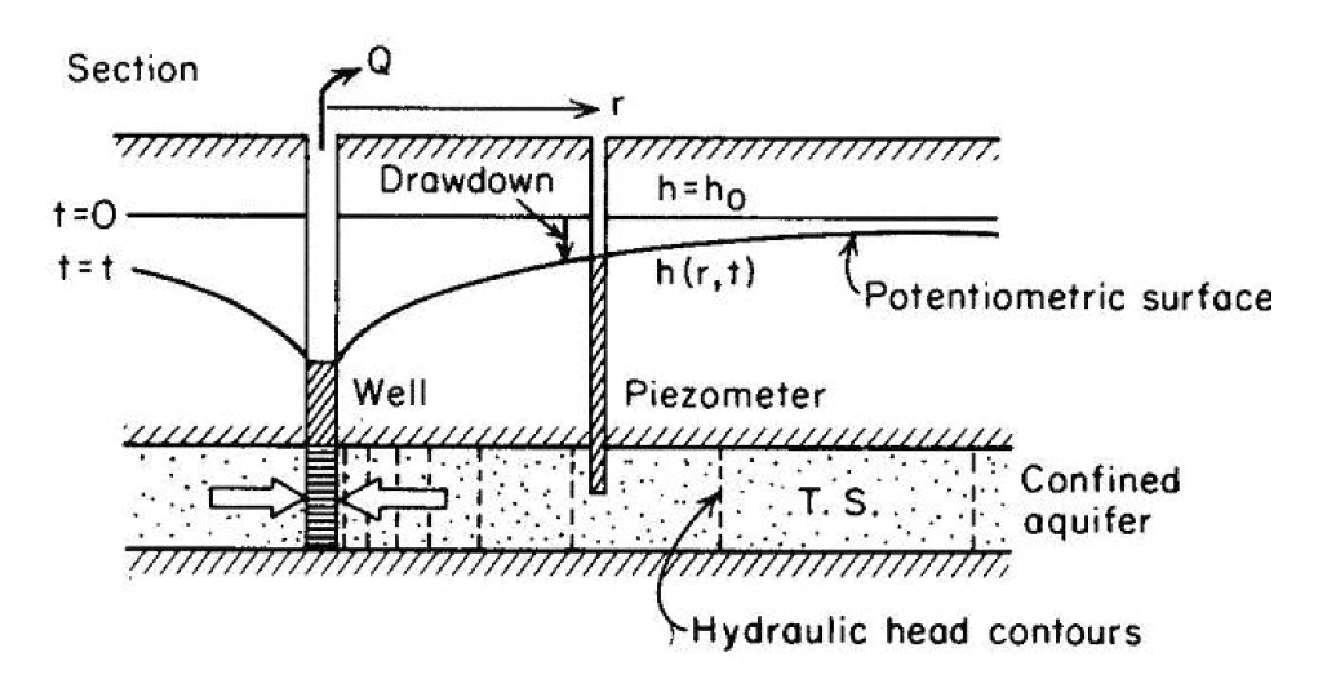
\includegraphics[width=0.5\textwidth]{C/figures/radial_flow_theiss_setup.eps}
\caption{Radial flow to a well in a confined aquifer (from Freeze and Cherry, 1979.}
\label{radial_flow_theiss_setup}
\end{figure}
The Theiss problem is used to verify the transient flow behaviour of GeoSys. Theiss (1935) presented an analytical solution for the transient drawdown in an infinite, uniform, isotropic and confined aquifer  of constant thickness (see Fig. \ref{radial_flow_theiss_setup}). The pumping well is assumed to fully penetrate the aquifer, have a neglible diameter and no well effects and to pump at a constant extraction rate. The initial hydraulic head is constant throughout the aquifer. This analytical solution is:
\begin{equation}
h_0 - h(r,t) = \frac{Q}{4\Pi T} W(\frac{r^2S}{4Tt})
\end{equation}
where $h_0$ is the initial hydraulic head [m], $h(r,t)$ is the transient hydraulic head [m] at time $t$ [s] at distance $r$ [m] from the pumping well, $Q$ is the constant extraction rate at the well [m$^3$s$^{-1}$], $S$ is the storage coefficient [-] and $T$ is aquifer transmissivity [m$^2$s$^{-1}$]. $W()$ is the Theiss well function.

The parameters used are: A model area of 1000 m times 1000 m with the well in the center, a constant thickness of 20 m, a hydraulic conductivity of 0.000578704 m/s and a storage coefficient $S_0$ of 1.000000e-005 (Caution: For the Theiss solution $S=M S_0$). This yields a transmissivity of 1000 m$^2$d$^{-1}$. Element sizes of 50 m are used, which are refined to 10 m and 2 m close to the pumping well. The pumping rate is -0.011574074 m$^{3}$s$^{-1}$, corresponding to 1000 m$^3$d$^{-1}$.

Results are shown in Figure \ref{radial_flow_theiss_top_view} in top view, also showing the grid used, and in Figure \ref{radial_flow_theiss_drawdown}, which depicts a comparison of the piezometric heads at observation points 30 m, 70 m and 100 m from the pumping well calculated by GeoSys and the analytical solution given by Theiss (1939). The correspondence is good, thus verifying radial transient flow.

\begin{figure}[htbp]
\centering
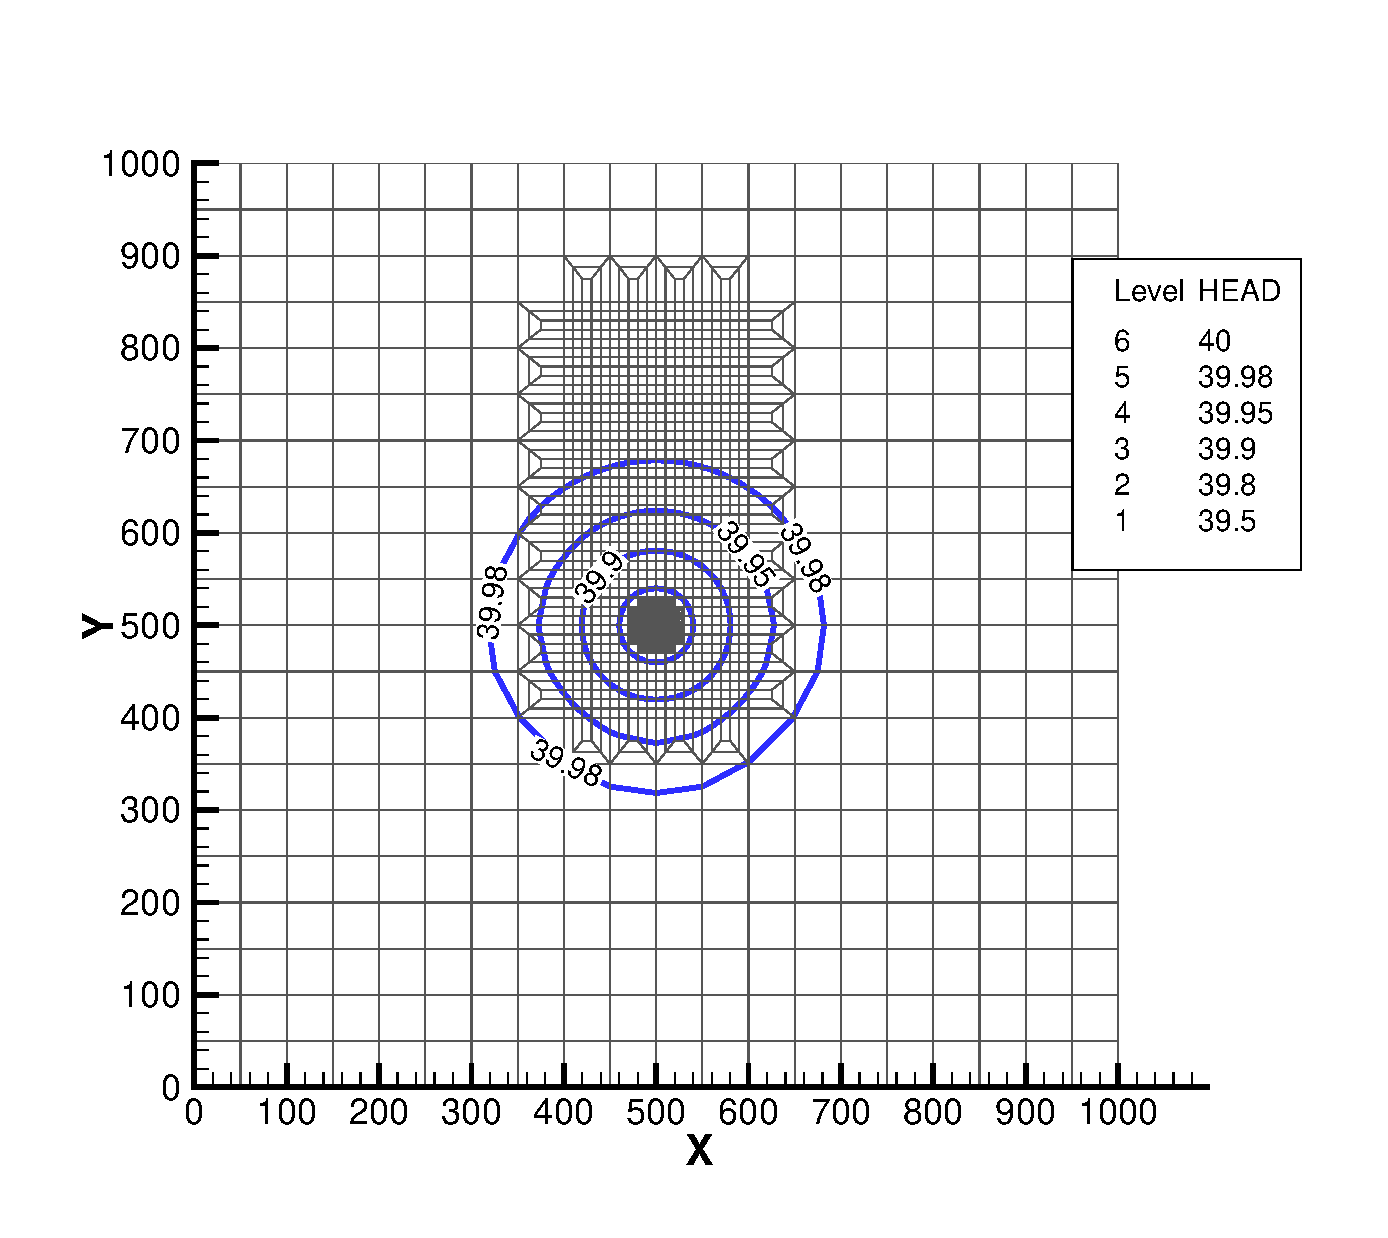
\includegraphics[width=0.5\textwidth]{C/figures/radial_flow_theiss_top_view.eps}
\caption{Radial flow to a well in a confined aquifer: Top view of the piezometric head.}
\label{radial_flow_theiss_top_view}
\end{figure}

\begin{figure}[htbp]
\centering
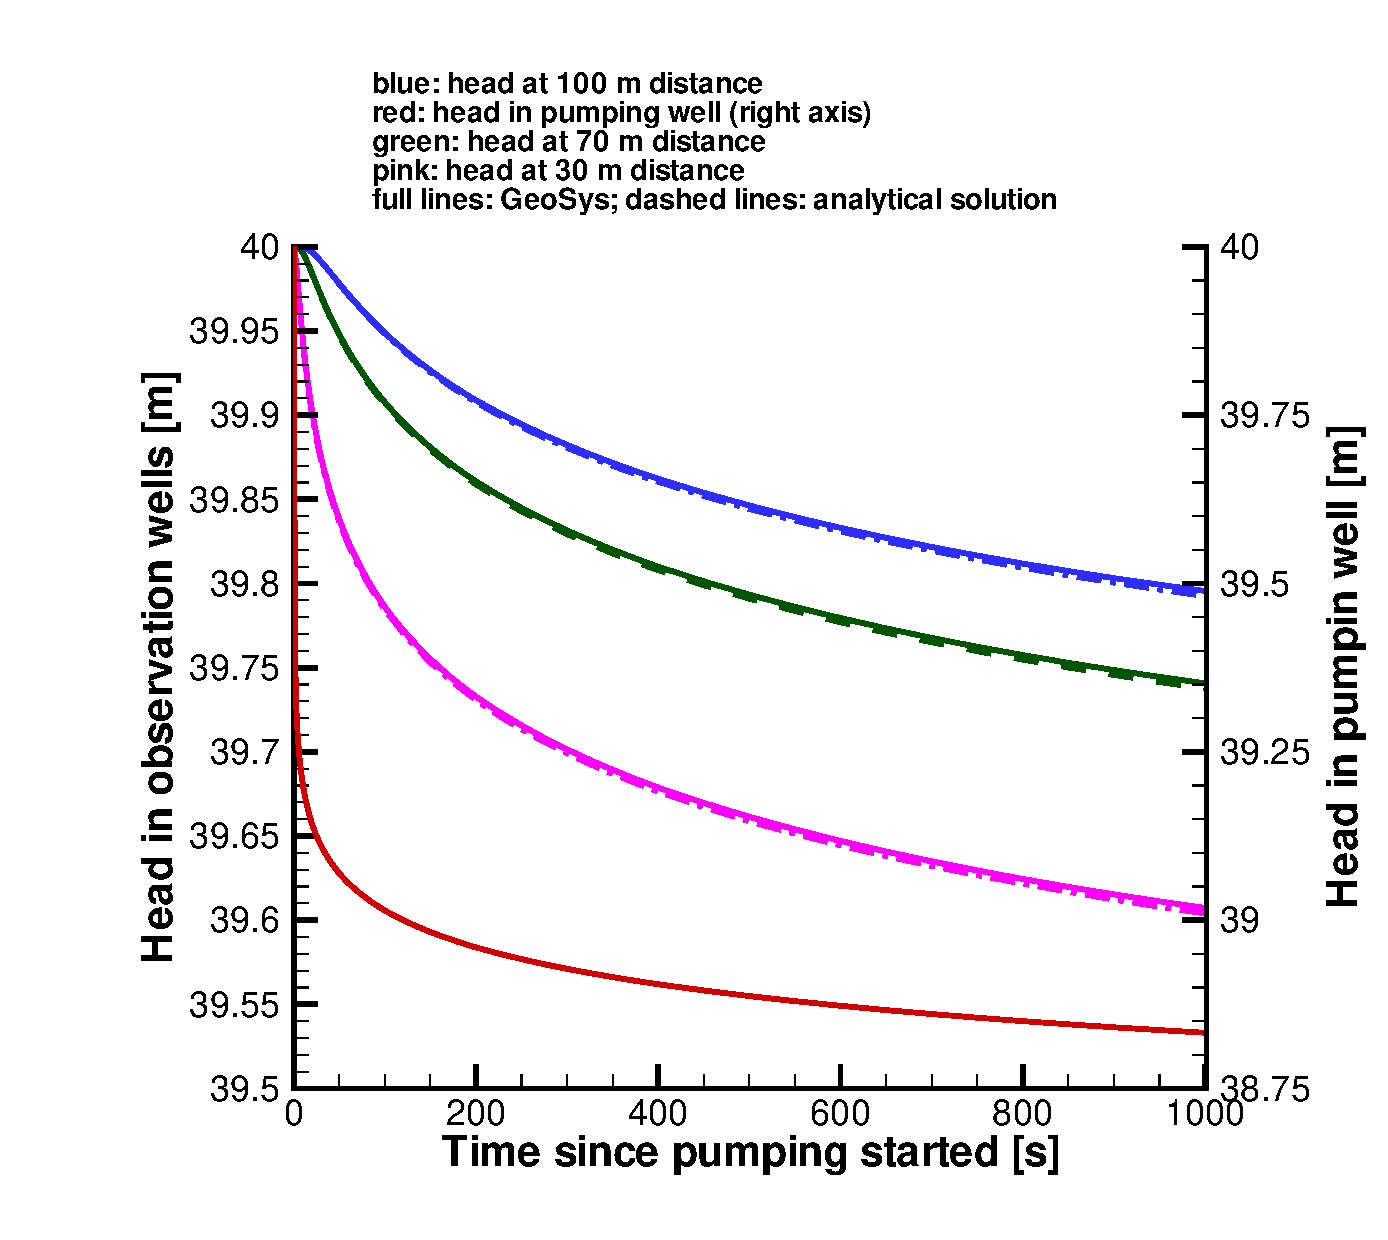
\includegraphics[width=0.7\textwidth]{C/figures/radial_flow_theiss_drawdown.eps}
\caption{Radial flow to a well in a confined aquifer: drawdown in the observation well, comparison to the analytical solution.}
\label{radial_flow_theiss_drawdown}
\end{figure}


\begin{table}[htbp]
\centering
\begin{tabular}{|l|l|l|}
\hline
Benchmark & Type & Path \\
\hline
\texttt{radial\_flow\_Theiss}& H &  benchmarks$\backslash$H$\backslash$radial\_flow\_Theiss  \\			
\hline
\end{tabular}
\end{table}

\subsection{Conservative Transport in radial flow}

This benchmark describes the behaviour of a conservative tracer injected in a fully penetrating well in a two-dimensional homogeneous confined aquifer.
The main purpose is to compare the numerical results of a conservative mass transport simulation without
any reactions in a radial flow field, with the approximate analytical solution for this problem that is given by Moench and Ogata (1981) and available in a computer program (LTIRD) provided by Javandel, Doughty, and Jsang (1984).

The aquifer is represented by a two-dimensional model of 300 m in both x and y direction with constant head boundary conditions at the four sides of the domain. The model is discretized in 30 rows and 30 columns with a constant width of 10 m. In order to obtain a better accuracy in the results, an area of 20 m around the injection well is further refined. The aquifer has an isotropic hydraulic conductivity K of 1.15741 $\cdot$10$^{-5}$ m s$^{-1}$, a porosity of 0.3 and injection rate Q 1.157407 $\cdot$10$^{-3}$ m$^{3}$ s$^{-1}$. Both longitudinal and transverse dispersivity have the same value  $\alpha_L$ $\alpha_T$ set to 10 m, while due to the model dimension and flow velocity, the diffusion coefficient is neglect. The physical aquifer parameters are summarized in Tab.~\ref{l_tab_benchmark_tracer_radial_flow}. The transport simulation is run for a period of 2332800 s with a time step length of 243 s.

\begin{table}[htbp]
\caption{Parameters used for benchmark HC$\backslash$radial\_flow\_transport}
\centering
\begin{tabular}{|l|l|l|}
\hline
parameter & value & unit \\
\hline
porosity $\Phi = n $  & 0.3&  --  \\			
\hline
hydraulic conductivity $K$ & 1.15741$\cdot 10^{-5}$ & ms$^{-1}$ \\ 			
\hline
injection rate $Q $ & 1.157407$\cdot 10^{-3}$ & m$^3$s$^{-1}$ \\ 	 			
\hline
storage coefficient $S$ & 0.0 & s$^{-1}$ \\
\hline
longitudinal dispersivity $\alpha_L$ & 10 &  m \\
\hline
transverse dispersivity $\alpha_T$ & 10 & m \\
\hline
total simulation time & 2332800 & s  \\
\hline
time step length  & 243 & s \\
\hline
\end{tabular}
\label{l_tab_benchmark_tracer_radial_flow}
\end{table}

\subsubsection*{Evaluation method}

Model results are compared to the approximate analytical solution from Moench and Ogata (1981).

\subsubsection*{Results}

Results of the tracer distribution along a polyline after 27 days are shown in Fig.~\ref{radial_flow_tracer_distibution} and the correspondence between anlytical solution and numerical simulation is very good.


\begin{figure}[htbp]
\centering
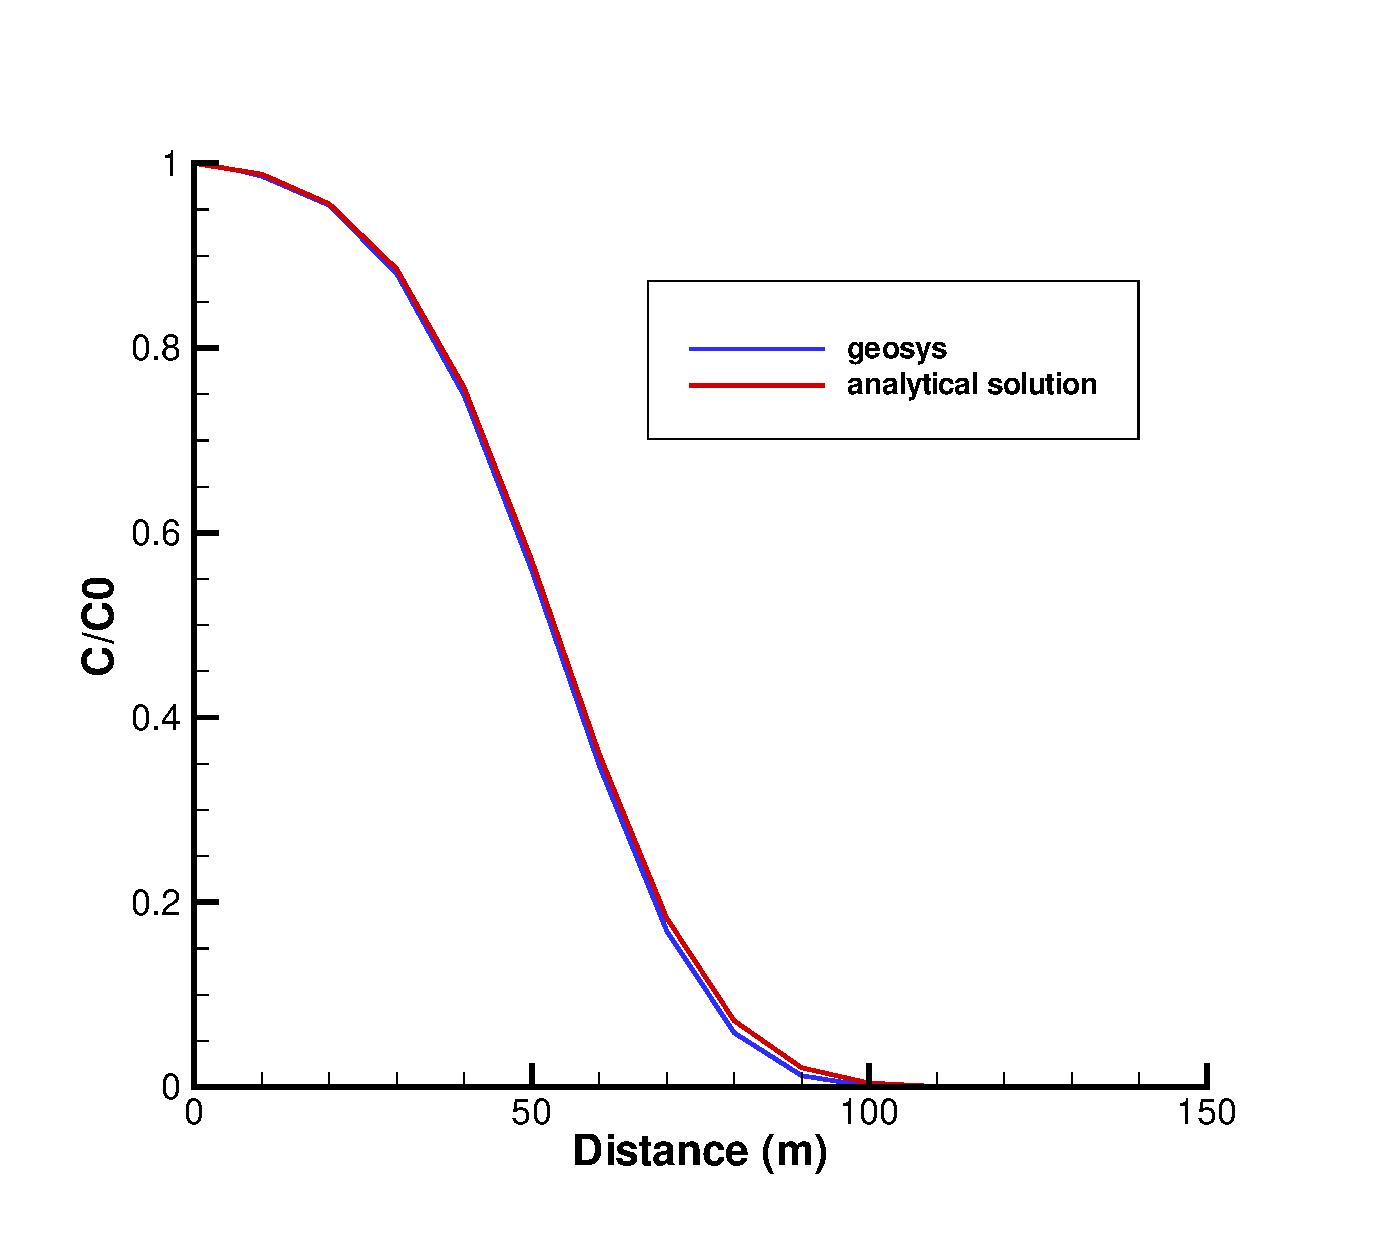
\includegraphics[width=0.5\textwidth]{C/figures/HC_RadialTransport_profile.eps}
\caption{Tracer distribution for radial diverging flow along a profile. Comparison of analytical solution and GeoSys/RockFlow results after 27 days of injection.}
\label{radial_flow_tracer_distibution}
\end{figure}



\begin{figure}[htbp]
\centering
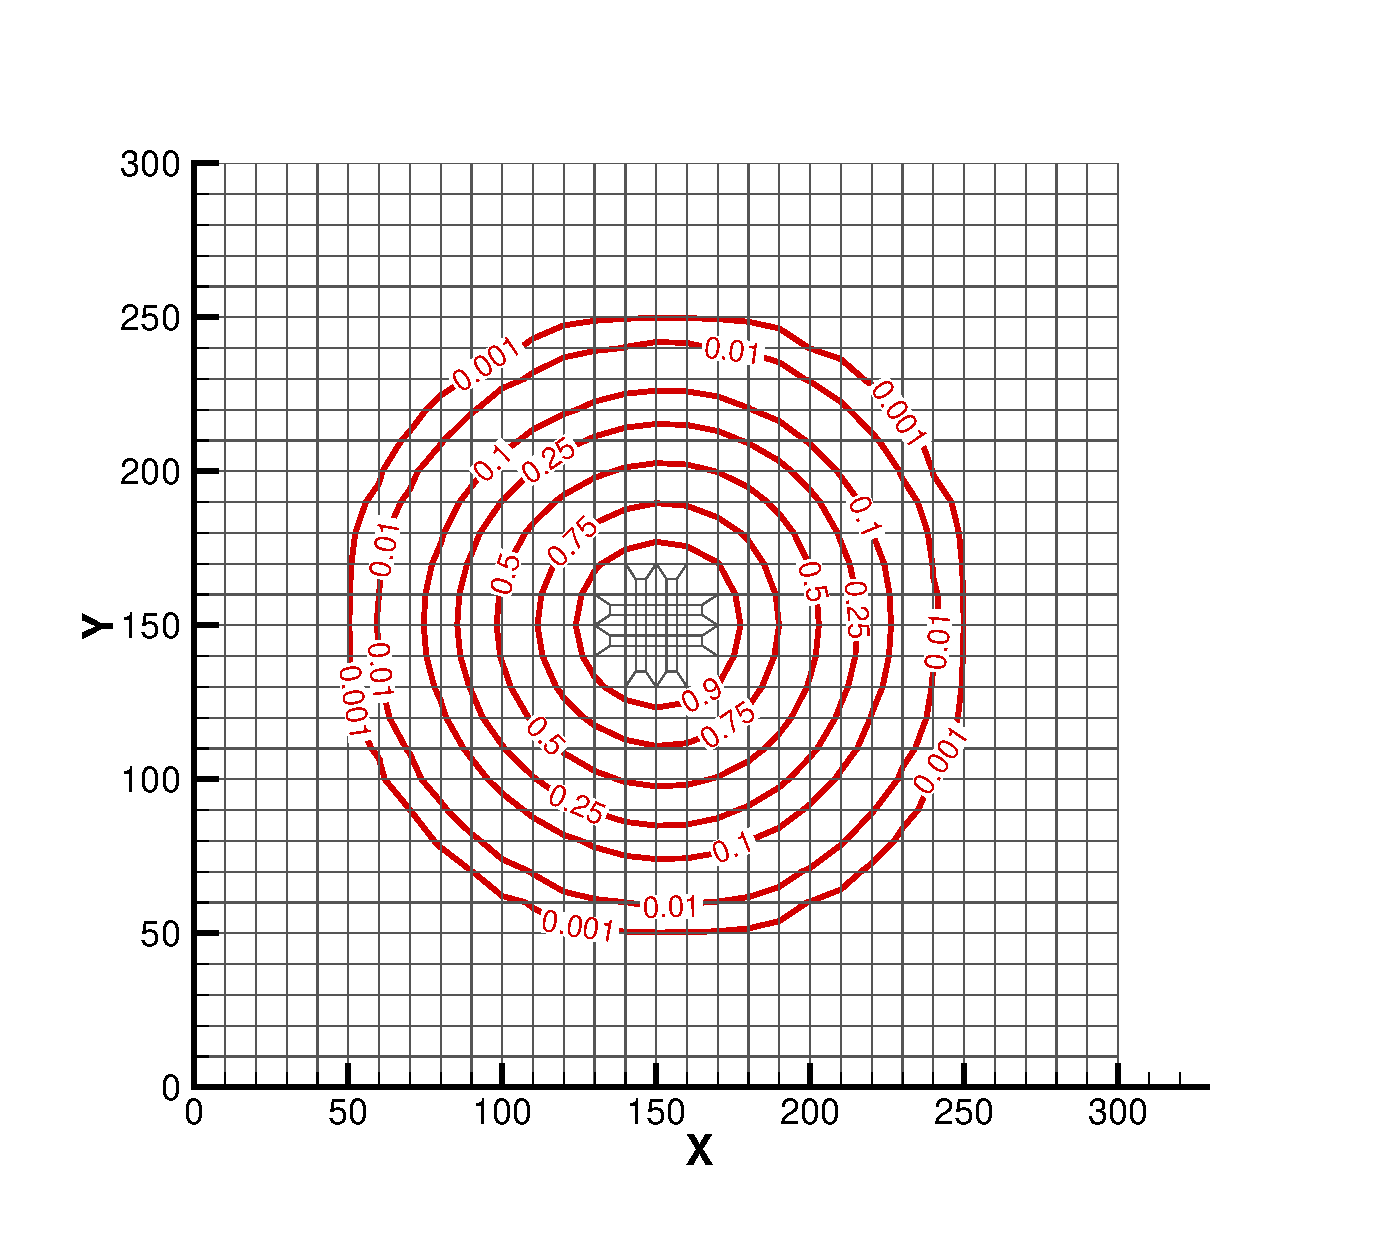
\includegraphics[width=0.5\textwidth]{C/figures/HC_RadialTransport_domain.eps}
\caption{Tracer distribution for radial diverging flow in top view. Isolines of tracer concentration from GeoSys/RockFlow results after 27 days of injection.}
\label{radial_flow_tracer_distibution}
\end{figure}


\begin{table}[htbp]
\centering
\begin{tabular}{|l|l|l|}
\hline
Benchmark & Type & Path \\
\hline
\texttt{radial\_flow\_transport}& HC &  benchmarks$\backslash$C$\backslash$radial\_flow\_transport  \\			
\hline
\end{tabular}
\end{table}
